\section{Resultados do modelo de detecção}
\label{sec:resultados_ml}

Esta seção apresenta os resultados do modelo de detecção, obtidos com o
protocolo das Seções~\ref{subsec:ml-protocolo} e
\ref{subsec:ml-protocolo-deteccao}. Eles vêm do \textit{dataset} Tour Perret, e
não das coletas da bancada da Seção~\ref{sec:resultados_infra}, porque essas
coletas duram horas e o modelo precisou de 14 dias de treino
(Seção~\ref{subsec:ml-res-treino}). O modelo final é o que o \textit{gateway} da
bancada executa, na forma da Seção~\ref{subsec:ml-res-borda}. Os erros de
previsão são em dB e foram calculados só nos quadros com RSSI observado.

\subsection{Comportamento da série}
\label{subsec:ml-res-serie}

A execução completa, do \textit{dataset} bruto aos resultados, foi refeita numa
cópia isolada do projeto, e todos os números se repetiram. No treino, a ACF do
nível do RSSI ficou perto de 0,8 em todas as defasagens até 40, sem cair, como
mostra a Figura~\ref{fig:ml-acf-pacf}. O teste KPSS rejeitou a
estacionariedade no nível, com estatística 9,342 e valor-p menor ou igual a
0,01, e não a rejeitou depois de uma diferenciação, com estatística 0,028 e
valor-p maior ou igual a 0,10. O modelo passou a usar $d = 1$.

\begin{figure}[htb]
	\centering
	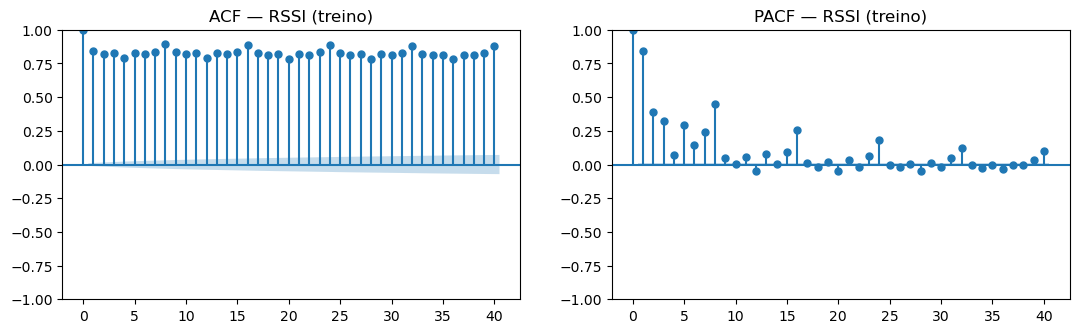
\includegraphics[width=0.95\textwidth]{tadaki/figuras/ml-acf-pacf.png}
	\caption{ACF e PACF do RSSI no treino}
	\label{fig:ml-acf-pacf}
	\legend{Fonte: elaborado pelos autores.}
\end{figure}

\subsection{ARIMA na série inteira}
\label{subsec:ml-res-inteira}

Entre as ordens candidatas, o ARIMA$(1,1,2)$ teve o menor RMSE na validação. No
teste, ele teve RMSE de 2,252, contra 2,874 do \textit{random walk}, ou seja,
22\% menos erro. O erro de previsão, porém, continuou autocorrelacionado, com
um pico na defasagem 8.

\subsection{Origem do erro na defasagem 8}
\label{subsec:ml-res-lag8}

O pico na defasagem 8 veio da troca de canal. O nó sensor usou oito canais, de
867,1 a 868,5~MHz, e o mesmo canal voltou 8 quadros depois em 49,4\% dos pares.
Cada canal teve um nível médio de RSSI próprio, de $-105{,}6$ a
$-101{,}3$~dBm no treino, como mostra a Figura~\ref{fig:ml-frequencias}. Na
defasagem 8, a diferença quadrática média entre quadros do mesmo canal foi de
1,47~dB, contra 3,08~dB entre quadros de canais diferentes. A causa física da
diferença de nível entre canais não foi medida.

\begin{figure}[htb]
	\centering
	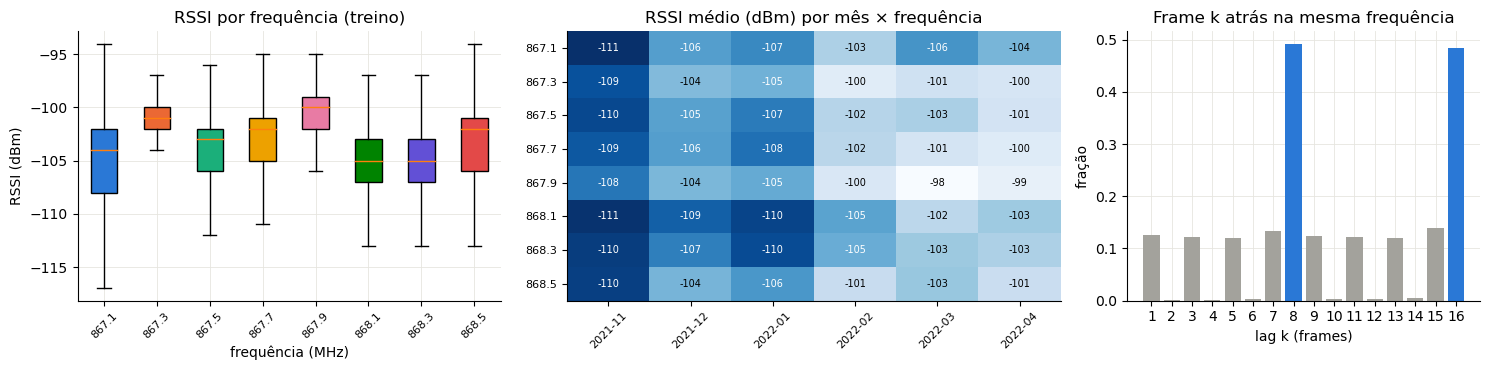
\includegraphics[width=\textwidth]{tadaki/figuras/ml-frequencias.png}
	\caption{RSSI por canal de frequência no treino, média mensal por canal e fração de pares no mesmo canal por defasagem}
	\label{fig:ml-frequencias}
	\legend{Fonte: elaborado pelos autores.}
\end{figure}

\subsection{ARIMA por canal e modelo final}
\label{subsec:ml-res-frequencia}

Com um ARIMA por canal, o erro caiu para menos da metade nas três medidas,
como mostra a Tabela~\ref{tab:ml-teste}. Variando a ordem um parâmetro de cada vez, o RMSE de
validação ficou entre 1,133 e 1,139 para todo modelo com ao menos um termo de
média móvel. Por isso o modelo final é o ARIMA$(0,1,1)$ por canal, que estima
só um coeficiente e a variância do ruído em cada canal. Avaliado uma única vez
no teste, ele teve RMSE de 1,091, praticamente o mesmo do ARIMA$(1,1,2)$ por
canal. Repetido no \textit{gateway} \texttt{100210b9}, o ARIMA por canal também
teve o menor erro, com RMSE de 1,018 contra 1,294 do \textit{random walk} por
canal.

\begin{table}[htb]
	\centering
	\caption{Erro de previsão no teste, em dB, no \textit{gateway} \texttt{17459c66}}
	\label{tab:ml-teste}
	\begin{tabular}{lrrr}
		\hline
		\textbf{Método} & \textbf{RMSE} & \textbf{MAE} & \textbf{Mediana de $|e|$} \\
		\hline
		\textit{Random walk} & 2,874 & 2,189 & 2,000 \\
		ARIMA$(1,1,2)$ na série inteira & 2,252 & 1,718 & 1,287 \\
		\textit{Random walk} por canal & 1,319 & 0,902 & 1,000 \\
		ARIMA$(1,1,2)$ por canal & 1,090 & 0,812 & 0,648 \\
		ARIMA$(0,1,1)$ por canal (modelo final) & 1,091 & 0,813 & 0,648 \\
		\hline
	\end{tabular}
	\legend{Fonte: elaborado pelos autores.}
\end{table}

A ordem dos métodos é a mesma pelo RMSE e pelo MAE, nos dois \textit{gateways}.
O tamanho do ganho, porém, depende da medida. Sobre o \textit{random walk} por
canal, o modelo final reduziu o RMSE em 17,3\%, o MAE em 9,8\% e a mediana do
erro absoluto em 35,2\% no \textit{gateway} \texttt{17459c66}, e em 21,2\%,
13,3\% e 36,6\% no \texttt{100210b9}. A diferença vem de o RSSI ser inteiro.
O \textit{random walk} por canal repete um valor inteiro e acerta o valor
exato em 37,5\% dos quadros do teste, enquanto o ARIMA prevê valores
fracionários e nunca acerta exatamente, mas tem erro típico menor, 0,65 contra
1,00~dB. A razão entre RMSE e MAE ficou entre 1,31 e 1,46 em todos os métodos,
o que é coerente com a cauda pesada do erro descrita na
Seção~\ref{subsec:ml-res-deteccao}. Na validação, o MAE escolheria a mesma
ordem que o RMSE em três de quatro casos. No caso restante, o ARIMA por canal
no \texttt{17459c66}, escolheria o próprio ARIMA$(0,1,1)$, empatado com o
ARIMA$(1,1,2)$ em 0,855~dB.

\subsection{Quantidade de dados de treino}
\label{subsec:ml-res-treino}

Com o ARIMA$(0,1,1)$ por canal, a partir de 14 dias de treino, cerca de 500
quadros por canal, o modelo atendeu ao critério da
Seção~\ref{subsec:ml-protocolo} em todos os períodos avaliados. Com 1 dia
atendeu em 62\% e com 7 dias em 88\%. O mesmo limite de 14 dias apareceu no
\textit{gateway} \texttt{100210b9}.

\subsection{Detecção de desvios do RSSI}
\label{subsec:ml-res-deteccao}

O erro de previsão na validação teve cauda mais pesada que a normal, com
curtose em excesso de 3,31. Com $c = 2{,}58$ da tabela normal, 1,47\% dos
quadros teriam passado do limiar, contra os 0,99\% esperados. O limiar
calibrado pelo quantil de 99\% ficou entre 2,4 e 4,1~dB nos oito canais, e o
piso de 1,5~dB não foi acionado. A taxa de alarmes falsos foi de 1,03\% na
validação e de 1,11\% no teste sem desvio, o que mostra que a calibração se
manteve fora da amostra.

A Tabela~\ref{tab:ml-deteccao} mostra a fração dos desvios sintéticos com ao
menos um alarme, em 300 posições do teste. Com essa taxa de alarmes falsos, um
desvio de 12 quadros teria ao menos um alarme por acaso em cerca de 12,5\% das
vezes. Desvios de 5~dB ou mais foram detectados em todas as posições quando
duraram 12 quadros, e em 91\% a 92\% quando pontuais. Desvios de 3~dB foram
detectados em 94\% a 99\% quando duraram 12 quadros, e em 42\% a 44\% quando
pontuais. Desvios de 2~dB por 12 quadros foram detectados em 72\%, e desvios
de 1~dB ficaram perto do acaso. Uma primeira execução, com 30 posições, deu a
mesma ordem de grandeza, mas com incerteza bem maior. O desvio de $+2$~dB por
12 quadros, por exemplo, foi detectado em 15 de 30.

\begin{table}[htb]
	\centering
	\caption{Desvios sintéticos detectados pelo ARIMA$(0,1,1)$ por canal, em porcentagem das posições do teste, com o intervalo de confiança de 95\% entre parênteses}
	\label{tab:ml-deteccao}
	\small
	\begin{tabular}{rcccc}
		\hline
		 & \multicolumn{2}{c}{\textbf{12 quadros (cerca de 1~h), 300 posições}} & \multicolumn{2}{c}{\textbf{1 quadro, 298 posições}} \\
		$\Delta$ (dB) & subida & queda & subida & queda \\
		\hline
		1 & 24 (20--29) & 28 (23--33) & 2 (1--5) & 3 (1--5) \\
		2 & 72 (66--76) & 72 (67--77) & 13 (10--18) & 17 (13--22) \\
		3 & 94 (91--96) & 99 (98--100) & 42 (36--48) & 44 (38--49) \\
		5 & 100 (99--100) & 100 (99--100) & 91 (87--93) & 92 (89--95) \\
		8 & 100 (99--100) & 100 (99--100) & 100 (98--100) & 100 (99--100) \\
		10 & 100 (99--100) & 100 (99--100) & 100 (99--100) & 100 (99--100) \\
		\hline
	\end{tabular}
	\legend{Fonte: elaborado pelos autores. No desvio de 1 quadro, 2 das 300 posições caíram em quadros sem RSSI observado e não entram na conta.}
\end{table}

\subsection{Comparação com um detector mais simples}
\label{subsec:ml-res-comparacao}

Aplicado o mesmo protocolo ao \textit{random walk} por canal, a taxa de alarmes
falsos no teste sem desvio foi de 0,79\% com a mesma regra e de 1,90\% com o
limiar um valor inteiro abaixo, contra 1,11\% do ARIMA. A
Figura~\ref{fig:ml-comparacao} mostra a fração de desvios detectados pelos
três detectores, com subida e queda somadas.

\begin{figure}[htb]
	\centering
	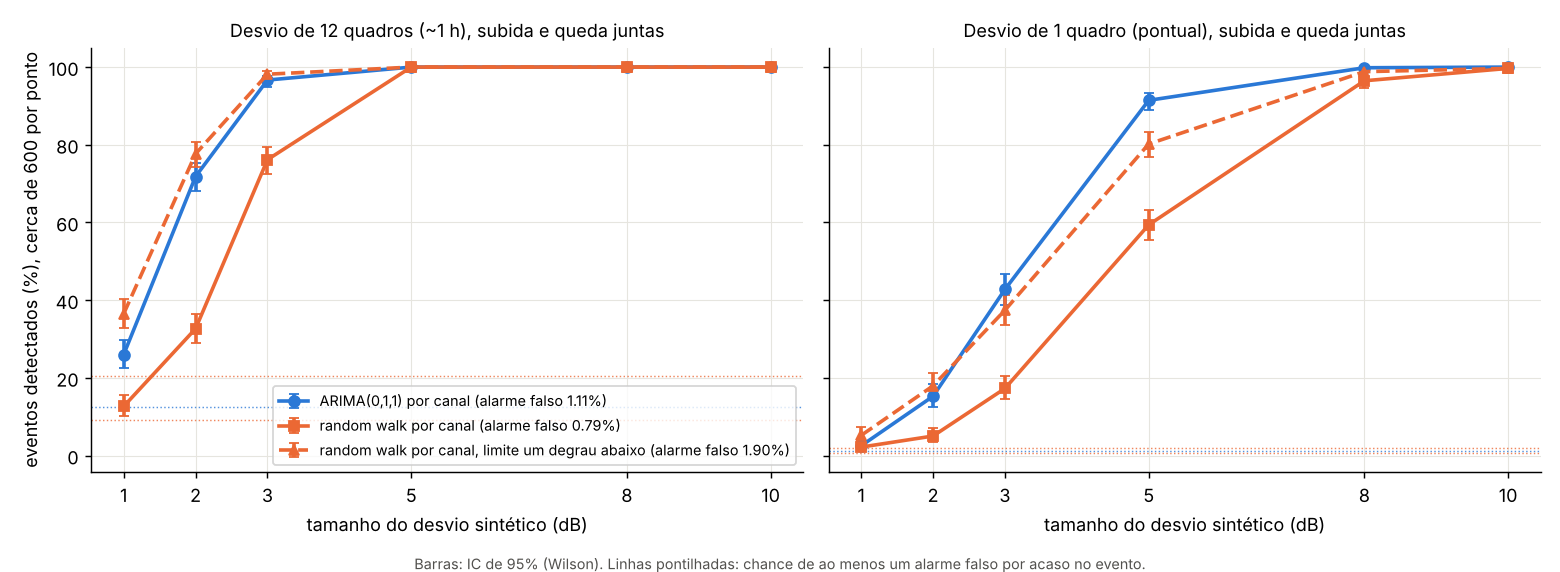
\includegraphics[width=\textwidth]{tadaki/figuras/ml-comparar-detectores.png}
	\caption{Desvios sintéticos detectados pelo ARIMA$(0,1,1)$ por canal e pelo \textit{random walk} por canal nas duas versões de limiar, por tamanho do desvio}
	\label{fig:ml-comparacao}
	\legend{Fonte: elaborado pelos autores.}
\end{figure}

Com a mesma regra, o \textit{random walk} por canal detectou menos que o ARIMA
nos desvios de 2 e 3~dB e nos de 1~dB por 12 quadros, por exemplo 31\% dos
desvios de $+2$~dB por 12 quadros, contra 72\% do ARIMA. Nos desvios pontuais
de 1~dB, os dois ficaram perto do acaso. Com o limiar mais baixo, ele se aproximou do
ARIMA nos desvios de 12 quadros, 75\% contra 72\% em $+2$~dB, mas com quase o
dobro de alarmes falsos. Nos desvios pontuais de 3 e 5~dB, o ARIMA detectou mais que as duas versões,
por exemplo 91\% dos desvios de $+5$~dB, contra 59\% e 80\%. Num desvio
persistente, o ARIMA continua alarmando. Com $+8$~dB por 12 quadros, ele alarmou
em 92\% dos quadros do desvio, e o \textit{random walk} por canal em 57\% a
59\%, porque este passa a prever o valor alterado já no quadro seguinte do
mesmo canal. A comparação não foi feita com a mesma taxa de alarmes falsos, já
que o ARIMA fica entre as duas versões do \textit{random walk}.

\subsection{Forma do modelo para o microcontrolador}
\label{subsec:ml-res-borda}

Com os coeficientes fixos, a recursão da Equação~\ref{eq:ml-borda} reproduziu a
previsão do ARIMA$(0,1,1)$ do \textit{statsmodels} em todos os 8.781 quadros do
teste, com diferença máxima de $1{,}8 \times 10^{-9}$~dB. A conta simples é,
portanto, o próprio modelo avaliado nesta seção, e não uma aproximação. Ela
guarda três valores por canal, o coeficiente $\alpha$, o limiar e a última
previsão.

\subsection{Requisitos atendidos}
\label{subsec:ml-res-requisitos}

O atendimento de cada requisito da Seção~\ref{sec:requisitos_ml} está resumido
no Quadro~\ref{qua:rastreabilidade_ml}. Os requisitos RF-M1, RF-M2, RNF-M2 e
RNF-M3 foram atendidos. O RF-M3 foi atendido com desvios sintéticos, e não com
ataques reais. O RNF-M1 foi medido só na validação.

\subsection{Limitações do modelo de detecção}
\label{subsec:ml-res-limitacoes}

Os resultados valem para um nó sensor, dois \textit{gateways} e um trecho de
203,7 dias. A magnitude que um ataque real provoca no RSSI não foi medida neste
\textit{dataset}. O nível do RSSI mudou em três degraus de cerca de 12~dB
dentro do treino, e a validação e o teste não têm degrau. Separar por canal não
reduziu o erro em dois dos cinco nós sensores. A ideia de separar por canal
surgiu depois da análise do erro do ARIMA na série inteira, que já tinha sido
avaliado no teste. A comparação entre detectores não foi feita com a mesma taxa
de alarmes falsos, e todos os desvios testados são sintéticos. O limite de 14
dias não corresponde à partida a frio de um nó sensor novo. A execução do
detector na placa, com o tempo por quadro e a conferência dos alarmes contra o
Python, não foi medida.
